\subsection{SSL Models' Architecture}
Modern SSL backbones share a similar architectural design that consists of two fundamental components: a feature extractor $\mathbf{F}$, typically implemented using CNNs, and a transformer encoder $\mathbf{E}$. The Transformer encoder is composed of $n$ layers which are denoted as $\mathbf{L}_i$. 

During the forward pass on downstream tasks, a raw waveform $\boldsymbol{x}$ first passes through the feature extractor to produce an initial representation $\boldsymbol{h}_0 = \mathbf{F}(\boldsymbol{x})$. Subsequently, $\boldsymbol{h}_0$ is processed through a series of transformer encoder layers. Each layer computes its output as $\boldsymbol{h}_i = \mathbf{L}_i(\boldsymbol{h}_{i-1})$.

After completing the forward pass, a sequence of hidden states $H = (\boldsymbol{h}_0, \dots, \boldsymbol{h}_n)$ is obtained. This set of hidden states is then used for downstream tasks.

\subsection{Layer Aggregation For Downstream Tasks}\label{sec:2_2}
The formulation of downstream tasks usually involves predicting $\boldsymbol{y}$ (i.e., class label, text, or speaker embedding) from waveform $\boldsymbol{x}$. This requires the SSL model, trained for the downstream task to have a probing head 
$p_\theta(\boldsymbol{y}|\boldsymbol{x})$ 
$ = \psi\left(\hat{\boldsymbol{h}}\right)$, 
where $\psi$ denotes the downstream model, 
$\theta$ are the model parameters
and $\hat{\boldsymbol{h}}$ are the hidden states of the model. In the simplest case $\hat{\boldsymbol{h}} = \boldsymbol{h}_n$, which we refer to as the \textit{last layer}. However, this approach does not utilize useful features from lower layers, leading to suboptimal performance. To address this issue, one can use learnable weights $w=(w_0, ..., w_n)$ to sum the representations from different layers

\begin{equation}\label{eq:weighted_sum}
    \hat{\boldsymbol{h}} = \sum_{i=0}^n w_i\cdot \boldsymbol{h}_i\ .
\end{equation}

\begin{figure*}[htbp]
    \centering
    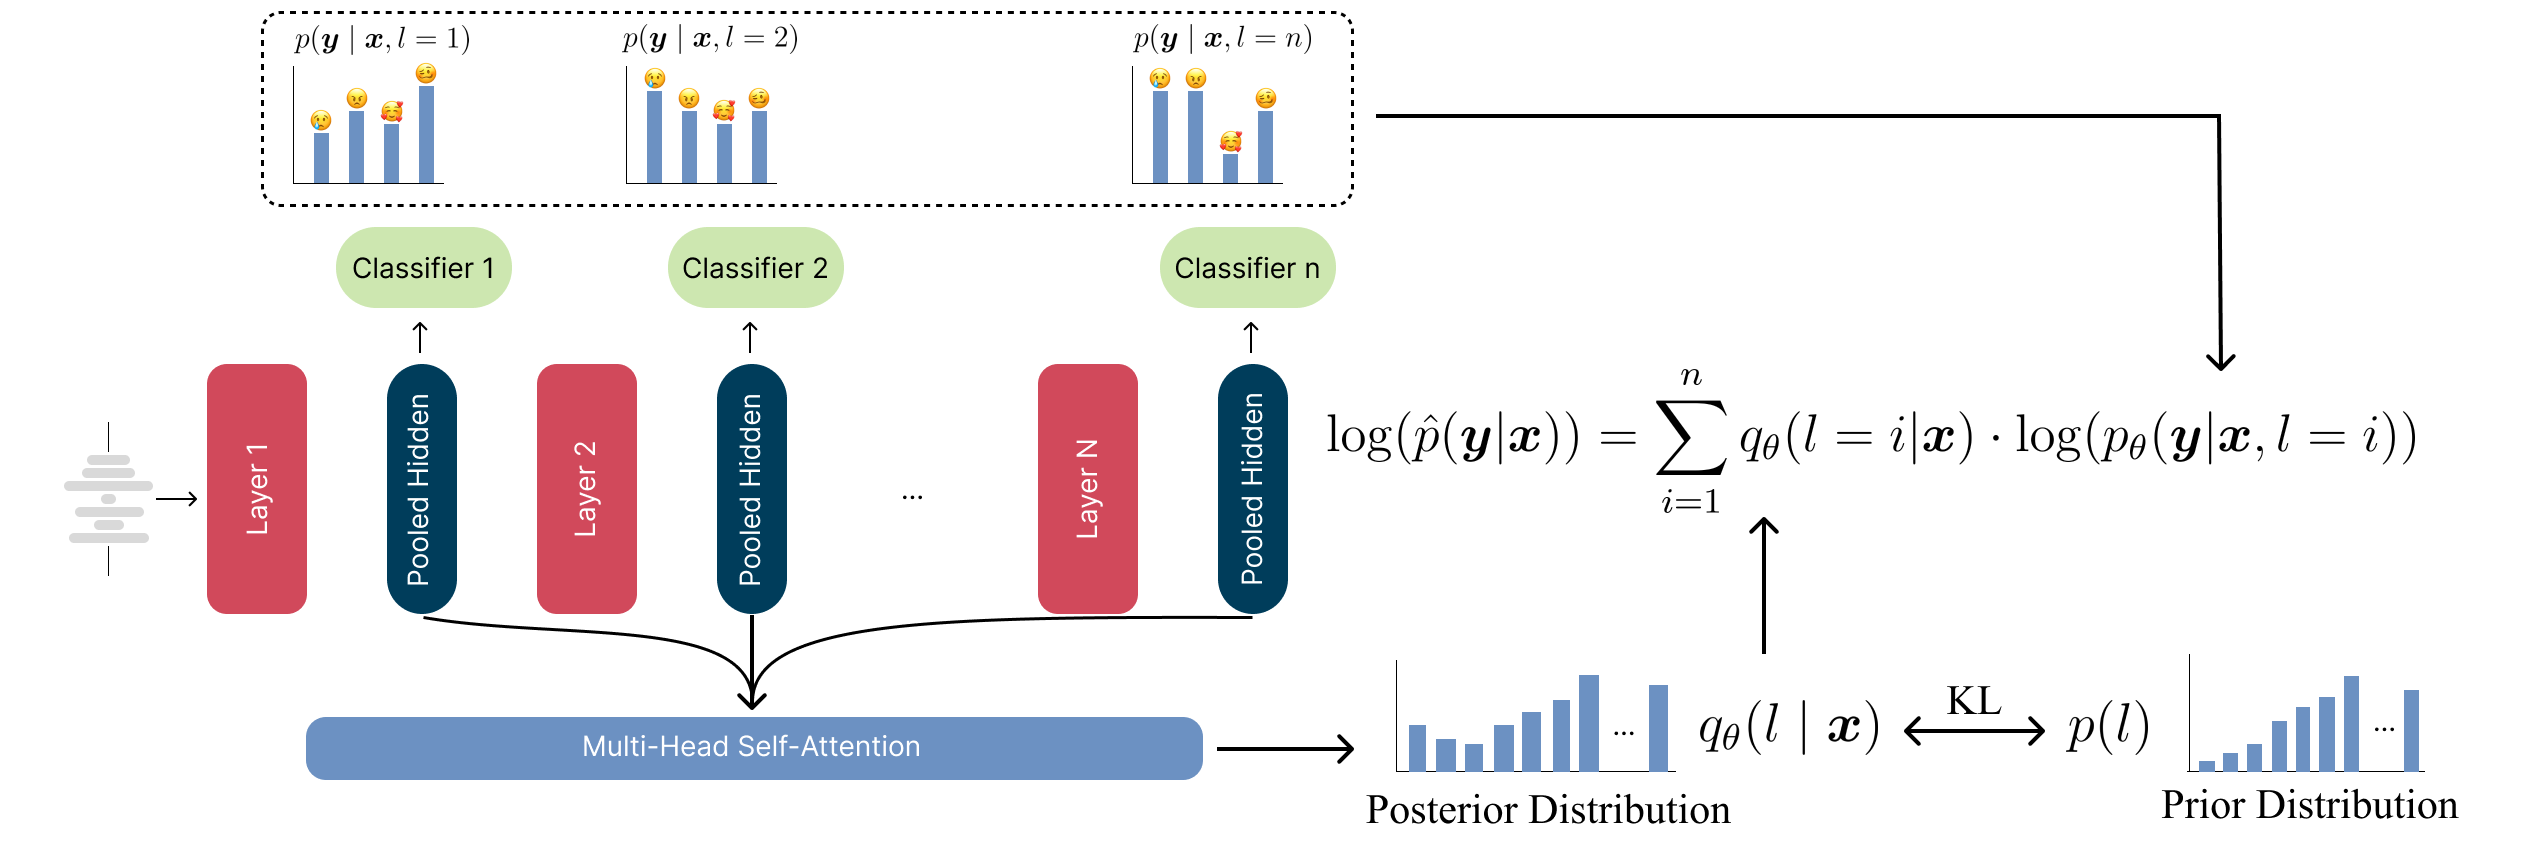
\includegraphics[width=0.99\linewidth]{figures/varan_illustration.png}
    \caption{Overview of the VARAN layer aggregation method.}
    \label{fig:varan}
\end{figure*}

\subsection{Efficient Fine-Tuning Methods}

The simplest approach to adapt a pre-trained model for a downstream task is full fine-tuning, where the model is initialized with pre-trained weights and all parameters are updated according to the training data. However, this approach often leads to challenges such as catastrophic forgetting \cite{kemker2017measuring} and representation collapse, particularly when the downstream task has limited training data. To address these issues, parameter-efficient fine-tuning methods have emerged as a compelling alternative. These methods not only reduce the number of trainable parameters but also help retain the valuable knowledge acquired during pre-training.

One prominent example of such methods is LoRA \cite{hu2021lora}, which offers an elegant solution by freezing the original model parameters and introducing low-rank matrices. Specifically, instead of updating the entire weight matrix $W$, LoRA decomposes the update $\Delta W$ into the product of two smaller matrices:
\begin{equation}
    \Delta W = A \cdot B,
\end{equation}
where $A \in \mathbb{R}^{d \times r}$ and $B \in \mathbb{R}^{r \times k}$ are trainable matrices, and $r \ll \min(d, k)$ represents the rank of the decomposition. By constraining the updates to a low-rank subspace, LoRA significantly reduces the number of trainable parameters while preserving the pre-trained model's knowledge. This enables efficient adaptation to downstream tasks without compromising the quality of the learned representations.
% In our work we focus on setup where we freeze feature extractor parameters and train only transformer encoder $\mathbf{E}$. We observe this setup being more stable and leading to better performance. 
